\documentclass[a4paper]{article}
\usepackage[utf8]{inputenc}
\usepackage[margin=0.8in]{geometry}
\usepackage{graphicx}
\usepackage{setspace}
\usepackage{float}
\usepackage{appendix}
\usepackage{tabu}
\usepackage{minted}
\usepackage{booktabs}
\usepackage{multirow}
\usepackage{amsmath}
\usepackage{xurl}
% use biblatex for refs
\usepackage[backend=biber]{biblatex}
\addbibresource{refs.bib}
% \usepackage{titlesec}
% last package to load
\usepackage[hidelinks]{hyperref}

\renewcommand{\familydefault}{\sfdefault}

% [minted] Set highlighting style
\usemintedstyle{tango}
\newminted{c}{breaklines=true}

\setlength{\columnsep}{0.5in}

\title{CM30075 Advanced Computer Graphics: Report}
\author{Candidate 21532}
\date{December 2022}
\begin{document}

\maketitle
\tableofcontents
\pagebreak

\section{Overview}
\subsection{Ray tracing}
Ray tracing is a method used in computer graphics to simulate light moving through a three-dimensional scene. This report accompanies a piece of software that uses ray tracing to produce an image using the famous Utah teapot model.

\subsection{Language and Libraries}
\paragraph{Rust} The software is written in Rust. Rust was chosen for this project because of its speed and support for multi-threading. It is also fairly similar to the more commonly-used C++, making the translation of the provided starter code fairly simple.

\paragraph{glam} Glam is a library that provides types and methods for vectors, a crucial foundations of graphics software. All types are also safe to use in parallel, perfect for ray tracing, and there is also a type for 3D transformations.

\paragraph{png} The software writes the pixel data produced into a .png image file. The png library allows this, and is easier than writing to a .ppm file and then converting it manually, despite the simplicity of the .ppm format. The library also handles the complexity of properly adjusting the colours if the image produced is too bright or dark.

\paragraph{acap} ``As close as possible'', abbreviated to acap, is a library that provides a number of different data structures which support search by proximity, including a KD tree. The library also includes methods for balancing and searching automatically.

\subsection{Structure}
The program is separated into multiple files, grouped by the types and traits that they contain. For types that implement a trait, their files are arranged into a folder named after the trait and the trait definition is in a file directly in the \texttt{src} folder. For example, the trait \texttt{Object} is defined in \texttt{src/object.rs} and the type \texttt{Sphere} that implements \texttt{Object} is defined in \texttt{src/object/sphere.rs}. Some files, like \texttt{src/photonmap.rs}, define multiple related types.\\

To run the program, you must have Rust installed: go to \url{https://rustup.rs/} to do so. Then the command \texttt{cargo run --package raytracer --release} may be used. The program will produce .png files as output in the root folder of the project.\\

The file \texttt{src/main.rs} contains the main function, which initialises the frame buffer(s), scene and camera before rendering the scene and photon map. It then calls the buffer to write its data to various files. \texttt{src/main.rs} also contains the function that creates the scene by specifying objects, their materials, and lights. See a summary of the contents of each file in \texttt{src/} in Table \ref{tab:projfiles}. Files inside folders in \texttt{src/} are excluded for brevity.\\

% TABLE =============================================================================================================
\begin{table}[h]
    \centering
    \caption{Project files in \texttt{src} folder}
    \label{tab:projfiles}
        \begin{tabular}{@{}l|l@{}}
            \toprule
            File & Contents \\ \midrule
            main.rs & Main control of program flow and scene building \\
            lib.rs & Project modules and Vertex type alias \\
            colour.rs & Colour type and associated functions and operators \\
            framebuffer.rs & FrameBuffer and Pixel types, and file writing functions \\ 
            fullcamera.rs & FullCamera type and functions, including scene rendering \\
            hit.rs & Hit struct which stores information about ray-object intersections \\
            light.rs & Light trait definition, links to `light/' \\
            linedrawer.rs & \textbf{[unused]} LineDrawer type and functions, used during development to debug Polymesh object \\
            material.rs & Material trait definition, links to `material/' \\
            object.rs &  Object trait definition, links to `object/' \\
            photonmap.rs & PhotonMap, Photon and PhotonHit types, functions and enums, including PhotonMap creation \\
            ray.rs & Ray type and functions and Reflectable trait \\
            scene.rs & Scene type and functions, including querying objects for their interactions with Rays \\
            \bottomrule
        \end{tabular}
\end{table}

\section{Basic Ray tracer}
\subsection{Camera}
In order to produce an image of a scene, a camera is used. The camera may be moved and rotated, its aperture adjusted, the number of samples per pixel altered, and an image size given. The camera position serves as the origin point for the rays that are fired through the image plane and into the scene. Each ray returns a colour which contributes to the final colour of the corresponding pixel it passes through.\\

\subsubsection{Multisampling} To create a more accurate image, multiple rays (samples) are fired through each pixel, and they all contribute equally to the final colour, as described in \cite{Cook1984multisampling}. The rays are fired with a small element of randomness to prevent them all taking the same path. Multisampling also allows the number of rays in the scene to be controlled. Although there are a greater number of rays per pixel, rays can be reflected or refracted (Section \ref{ss:reflandrefr}) stochastically (also called ``Russian roulette'' in the context of photons) rather than ``branching'', which generates multiple new rays from an intersection. Generating multiple new rays can result in a much greater quantity of them in the scene, slowing down the runtime considerably.\\

In addition, this technique allows for depth of field in the output image (Section \ref{ss:depthoffield}).\\

\subsubsection{Multithreading}
The camera runs a function `render()' to produce the data for each pixel. The image is divided into 8 sections vertically so that 8 threads can run at the same time on 8 cores, speeding up the rendering time massively. Rust was built to make parallel computing easy, and ray tracing lends itself well to parallel execution. Memory safety, mutexes etc. are all taken care of by Rust, and provide a huge optimisation. When a thread has computed a colour for the pixel it is working on, it send the pixel position, colour and depth to a receiver via a channel, and the receiver picks each pixel off the channel and writes it to the \texttt{FrameBuffer}. After all the sending threads finish, the receiver thread finishes too, and the frame buffer contains the complete image.

\subsection{Basic Objects}
The software supports a few different types of object. An object, no matter its type, must be able to determine if a given ray will intersect with it, and if so, where the intersection will be, what event happens at the surface (ray is reflected, absorbed or transmitted), and so on.

\paragraph{Spheres} The most simple is the sphere, since the test for an intersection is easy. The parametric equation of a sphere is used, along with the ray, to determine whether there is an intersection and its position. Spheres are commonly used to showcase different materials in graphics, as they have uniform shape with varying surface normals.

\paragraph{Plane} An infinite plane can be expressed as a surface normal and a point in the plane. Using the implicit equation, the intersection test is very basic geometry. The plane is useful during debugging to show the shadow of other objects, which places them in relation to one another.

\paragraph{Polymesh} A polymesh is a set of primitives (triangles) that together form a model, with famous examples being the Stanford bunny, Utah teapot and Stanford dragon. The software is capable of interpreting polymeshes from files in the ``kcply'' format (as opposed to the standard .ply format) that are zero or one-indexed. Each triangle is defined as a trio of vertices in the file. The intersection testing for a polymesh is intensive and complex, as it includes smoothing by using vertex normals. In order to achieve this, normals for each triangle and vertex are computed during the creation of the object, requiring several passes through the triangles.\\

Intersections with triangles are computed by using Barycentric coordinates and the M{\"o}ller-Trumbore intersection algorithm \cite{Moller1997mtalgo}. This allows the vertex normals to be combined at a location where the ray hits according to the proximity of the intersection with each vertex, producing a smooth looking object in the output. The program uses the Utah teapot data to showcase this. This intersection test is time consuming, as every single triangle must be checked for an intersection with every ray, but produces a nicer image. This can be seen in Image \ref{fig:smoothing}.

\paragraph{Triangles} A single triangle can be used to form a plane with finite size using the same intersection algorithm as the polymesh, which is useful for when it's not worth the time to write a whole file in kcply or ply format. The triangle objects are used in the program to form the walls of a Cornell box.

\subsection{Lighting}
\subsubsection{Lights}
Lights need to be used in order to realistically colour objects and their shadows in 3D space. A light emits light in one or many directions of some given colour. The light colour will alter the the colour that appears on each surface in the image.\\

The most basic type of light is the \texttt{Directional} light, which simulates a light source that's very far away (like the sun). The direction from any point on any surface is always the inverse of the light's direction. The problem with using a directional light is the lack of control over the light's position. A \texttt{Point} light is a point in space that emits light equally in all directions. This is excellent for scenes such as the Cornell box, where the walls and ceiling of the box would occlude a directional light from above.\\

The traditional Cornell box uses an area light, which is yet more realistic than the point light. However, using an area light incurs significant computational cost, and is out of the scope of this project.\\

\subsubsection{Occlusion}
In order for shadows to be more realistic, there needs to be some way to make sure that when an object comes between a surface and the light source, the object casts a shadow. This is called occlusion, and is controlled by the \texttt{Scene} using the \texttt{shadow\_trace()} function.\\

\subsection{Materials}
The appearance of an object is affected by the light that hits it interacting with its \texttt{Material}. The material controls the properties and colours of a surface. One material that tends to be used for debugging that does not interact with incoming light is the \texttt{NormalShading} material, where the colour output for each point is a function of the surface normal. It is useful especially when developing the polymesh object, as the surface normals are easy to get wrong. During development, I often ended up with inverse normals or normals of non-unit length, and the normally shaded material makes it very easy to debug that issue. This material can be seen in Image \ref{fig:normalshading}.\\

Other materials include metal, glass (dielectric) and Phong materials. Incoming light gets reflected, transmitted or absorbed, according to the material, and for each ray fired at a material, a colour is returned. Since this process is recursive for reflective objects like metal (as the pixel colour needs to have contribution from the objects in the reflection, too), there is a maximum recursion depth. As mentioned above, in situations where a ray may reflect or refract, the outcome is determined based on probability. Reflection and refraction are not features of the basic ray tracer and are discussed in Section \ref{ss:reflandrefr}.\\

Diffuse (matte) surfaces scatter incoming rays in a random direction, resulting in a uniform surface that is not glossy or specular. This is often called Lambertian, and is one part of the Phong lighting model \cite{Phong1975lighting}. The Phong material was developed to approximate light more accurately than previously available by combining three terms: ambient, diffuse and specular. The result is a plastic-like material that shows the form of the object. The ambient term is the darkest colour, and applies to the entire object. The diffuse term provides the mid-tone, depending on the location of the light sources. The specular term depends on the position of the camera (viewer) in relation to the surface, and is the brightest term. The Phong lighting model may look unrealistic by modern standards, but was groundbreaking in its time.\\

\section{Feature-Rich Rendering}
\subsection{Reflection and Refraction}\label{ss:reflandrefr}
Reflection and refraction occur when a ray hits a material that is \texttt{Metallic} or \texttt{Dielectric} (glass-like). Reflection occurs when a ray hits a reflective surface, at which point a new ray is created from the hit point in the reflected direction about the surface normal. If that ray hits another reflective surface it may spawn yet another new ray until the recursion depth is reached (to prevent infinite ray bouncing). If the ray hit a diffuse surface, the surface colour contributes to the initial hit (as if an object is in a mirror). For a metallic material, all rays are reflected, but the direction may be affected by the \texttt{roughness} field. The rougher the material, the more the direction of the reflected ray is altered by randomness. This is seen  in the \texttt{interact()} function on \texttt{Metallic}:

\begin{minted}{Rust}
    let r = (hit.incident.direction.normalize().reflect(hit.normal)
            + self.roughness * random_in_unit_sphere())
        .normalize();
\end{minted}

Refraction occurs according to Snell's Law: the angle of a light ray changes when crossing the boundary between media with different refractive indices. Snell's Law is given by: $\frac{\sin \theta_{1}}{\sin \theta_{2}} = \frac{n_{1}}{n_{2}}$ where $\theta$ is the angle of incidence and $n$ is the refractive index of the material.

\subsubsection{Fresnel Term} When an observer views a dielectric object directly (direction is close to opposite the surface normal), they can see straight through it. For example if you stand in a swimming pool and look down, you can see through the water. However, if you look out across a lake or ocean, you cannot see through it: this is due to the angle of observation being close to perpendicular to the surface normal. In this example, a large body of water acts like a mirror when viewed in this way. Fresnel determined exactly how the ability of a surface to reflect light varies with incident angle.\\

This phenomenon can be simulated by introducing the Fresnel equations into the \texttt{Dielectric} material as described in \cite{Suffern2016ray}, but a good approximation may be used instead: Schlick's approximation \cite{Schlick1994approx} for reflectance. The following function returns the reflectance probability of the material given the cosine of the incident ray and refractive index:

\begin{minted}{Rust}
    fn reflectance(cos: f32, index: f32) -> f32 {
        let r0 = ((1. - index) / (1. + index)).powi(2);
        r0 + (1. - r0) * (1. - cos).powi(5)
    }
\end{minted}

This effect can be observed in Image \ref{fig:fresnel}. Notice how in the right image, around the sphere edges, there is a faint reflection of the environment visible.

\subsection{Constructive Solid Geometry}
CSG is a technique used very often in modelling to create complex shapes from basic 3D primitives. A CSG is a binary tree of objects and their relationships. For example, two intersecting spheres may have the operation \texttt{Op::Union}, resulting in a single object that combines the areas bound by both. The relationship between objects can be \texttt{Op::Union}, \texttt{Op::Intersection} or \texttt{Op::Difference}. These three cases are shown in Image \ref{fig:csgtypes}.

\subsection{Quadratic Surfaces}
Quadratic surfaces are surfaces defined by the following: $ Ax^{2}+By^{2}+Cz^{2}+Dxy+Exz+Fyz+Gx+Hy+Iz+J=0 $ and are most commonly an ellipsoid, cone, paraboloid or hyperboloid. Alternatively, they can be expressed as:
\begin{align*}
    &
    \begin{bmatrix}
        x & y & z & 1 \\
    \end{bmatrix}
    \begin{bmatrix}
        a & b & c & d \\
        b & e & f & g \\
        c & f & h & i \\
        d & g & i & j 
    \end{bmatrix}
    \begin{bmatrix}
        x \\
        y \\
        z \\
        1
    \end{bmatrix} = 0
\end{align*}

The \texttt{Quadratic} object stores coefficients $a$--$j$ as the array \texttt{coeffs} instead of as a $4*4$ matrix to prevent redundancy. Admittedly, this makes the intersection test and transformation very verbose. With more time, there is definitely room to make this object implementation more streamlined. An example of a common quadratic surface case is seen in Image \ref{fig:quadsurface}: an ellipsoid.

\subsection{Depth of Field}\label{ss:depthoffield}
Depth of field refers to the fact that some objects appear sharp and others appear blurry, according to the distance of the objects from the camera's focal plane. This cannot be observed when the camera acts as a pinhole camera with a infinitely small aperture, as the basic camera does. Depth of field makes an image appear more realistic, simulating a non-pinhole camera, and the strength of the blur produced is controlled by the camera's aperture. A pinhole camera may still be simulated by using an aperture of $0.0$.

\subsubsection{The Thin Lens model}
The ``Thin Lens'' model, taken from the field of optics, makes some generalisations about the physics of a real lens by assuming the lens' width is negligible compared to the distance from the lens to the focal plane. The focal plane is the same as the image plane in this implementation, as it locates the pixels of the final image, which should be in focus, relative to the 3D scene. The lens is implemented as a circular disc around the camera's position within which the rays are fired from. The greater the aperture, the more spread out the rays travelling towards a given pixel are, and the less "accurate" (sharp) the final colour will be if the colour comes from an object far away from the focal plane.\\

The offset of rays by some amount within the lens disc is achieved by generating a random vector within a unit disc and multiplying it by the camera's aperture. The direction of the ray also needs to be adjusted, otherwise it will not point exactly to the correct pixel, and objects that should be in focus would appear blurry. The correct effect can be seen in Image \ref{fig:depthoffield}, where the focal plane intersects with objects roughly in the middle of the box.

\section{Photon Mapping}
Photon mapping is a technique used to more accurately simulate real light by tracing rays (photons) from light sources into the scene and then using the resulting information about their paths in the rendering stage, as described in \cite{Jensen1996photonmaps}. By using photon mapping, some important visual effects can be shown in renders, like caustics through a glass object or colour bleeding from matte surfaces.

This program uses multiple photon-related types for this, including \texttt{PhotonMap}, \texttt{PhotonHit} and \texttt{Photon}. There are also relevant methods added to \texttt{FrameBuffer} and \texttt{Material}. Photon mapping is done in two stages and is thus called a two pass algorithm: first the \texttt{PhotonMap} is generated, and then it is used during the rendering stage in conjunction with the more basic ray tracing methods.

\subsection{Photon Generation}
The first pass is the generation and firing of \texttt{Photon}s. Photons are fired from each light source into the scene which, in the case of the \texttt{Point} light, means in all directions. Photons that hit an object are recorded as \texttt{Type::Direct} photons in a \texttt{PhotonHit}. Depending on the material of the object, a new photon might be generated that is \texttt{Type::Indirect} - this occurs when a photon hits an object and is \texttt{Interaction::Reflected} or \texttt{Interaction::Transmitted}. For each direct hit, a \texttt{Type::Shadow} photon is also fired along the same trajectory as the original photon, in order to record the location where that direct hit casts a shadow. This is used for optimisation during rendering.

\subsubsection{Events}
The type of event that occurs when a photon hits a material is recorded with the enum \texttt{Interaction}, which is returned when the \texttt{interact()} function is called on a material. It is specifically useful for matching against when each type of event is treated differently. For a material like \texttt{Dielectric}, the interaction could be transmission or reflection, determined stochastically.

\subsubsection{Dielectric shadows}
A side effect of introducing the different types of interactions with materials, the \texttt{shadow\_trace()} function was augmented to increase the accuracy of glass shadows, as seen in Image \ref{fig:glassshadow}. If a ray is transmitted, no shadow is produced: this means that the glass sphere produces a shadow that shows off the Fresnel behaviour with a darker ring where rays are reflected around the edges.

\subsection{Photon Map}
Photon hits are stored in a photon map in order to be accessible during the rendering phase. The preferred data structure for this is the KD tree. This is used because ``In order for the photon-mapping algorithm to
be practical, the data structure has to be fast when it comes to locating
nearest neighbors in a three-dimensional point set.'' \cite{Jensen2001RealisticIS}. A great library for this is the \texttt{acap} library, containing the \texttt{KdTree} type. The library has support for a ``k-closest neighbours'' search, perfect for photon mapping. A visualisation of a complete photon map is seen in Image \ref{fig:pmap}, which uses the same scene as Image \ref{fig:glassshadow}. This visualisation shows a sort of irradiance estimate for the scene by finding the closest photons in a radius around the point in question and taking an average of their intensity. The more photons you fire, the more accurate the photon map is, but the longer it takes to construct.

\subsubsection{Caustics}
Caustics are generated separately from the normal photon map, as a very large number of photons is required to create a convincing effect. A caustic photon map is treated slightly differently in the code, for example by using the \texttt{build\_caustics()} function instead of the \texttt{build()} function. Caustics occur at refractions or specular reflections, but this program only creates refracted caustics.\\

The caustic map is used in a different way to the standard photon map in that it can be directly visualised instead of meshed into the rendering phase. This code achieves this by creating a normal rendered frame buffer and combining it with a frame buffer containing the visualisation of the caustics directly with the \texttt{add\_caustics()} function of \texttt{FrameBuffer}. This effect is seen for a large glass sphere in Image \ref{fig:glasscaustics}.

\subsection{Rendering}
The following is not implemented in the submitted software, and the only ``rendering'' is the naive addition of a caustic photon map, which is very limited in practice.\\

The photon map(s) are used during the rendering stage to produce a more accurate image. Different types of ray path are handled differently, and are rendered either accurately or inaccurately depending on how much they contribute to the image. The types of ray path are distinguished according to the types of interactions photons have on their path from the light: photons that have hit specular surfaces and been reflected are treated as a separate case to a photon that has directly been absorbed from the light.\\

The photon map provides an estimate for the amount of energy (radiance) entering and leaving each part of the scene. This is computed by integrating over an area of some radius centering on the point in question, according to the hits recorded in the photon map. This is similar to the method used to directly visualise the caustics map described above. All of this serves to complete each component of the rendering equation, which ``forms the mathematical basis for all global illumination algorithms'' \cite{Jensen2001RealisticIS}, given as:

\begin{align*}
    L_{o}(x, \overrightarrow{\omega}) = L_{e}(x, \overrightarrow{\omega}) + L_{r}(x, \overrightarrow{\omega})
\end{align*}

This equation describes the outgoing radiance at a point ($L_{o}$) as the sum of the emitted and reflected radiances ($L_{e}$ and $L_{r}$). The emitted radiance for objects that do not give off light is zero, so we just need to work out the reflected term, which can be expressed as the sum of four integrals that are evaluated separately. The four contributions are: direct illumination from lights, specular reflections, caustics and indirect illumination (photons that have bounced diffusely at least once) \cite{Jensen1996photonmaps}.\\

\paragraph{Direct illumination} is computed accurately (without the photon map) when the photon map indicates that the area in question is directly illuminated and there are no shadow photons near-by. Inaccurately, it can be taken directly from the radiance estimate by taking photons from the photon map.

\paragraph{Specular reflections} are computed without the photon map, as the photon map is not accurate enough to give a nice image.

\paragraph{Caustics} are computed using \textit{only} the information in the caustic photon map, as traditional ray tracing struggles to simulate these effects at all (although it is possible).

\paragraph{Indirect illumination} is where the information in the photon map is really valuable. For non-accurate evaluation, the radiance estimate from the photon map is fine, but for accurate evaluation this needs to be combined with the traditional ray tracing to produce a convincing effect.\\

The combination of these approaches allow for caustics and diffuse colour bleeding, and well as the soft illumination that comes from diffuse photon bouncing, that are not typically seen in traditional Monte Carlo style ray tracing. A particularly famous application of caustics is the simulation of liquids, as seen in Image \ref{fig:cognac} \cite{Jensen1996photonmaps}.

\pagebreak
\printbibliography
\pagebreak
\appendix
\section{Images}

%polymesh smoothing on/off
\begin{figure*}[h]
    \centering
    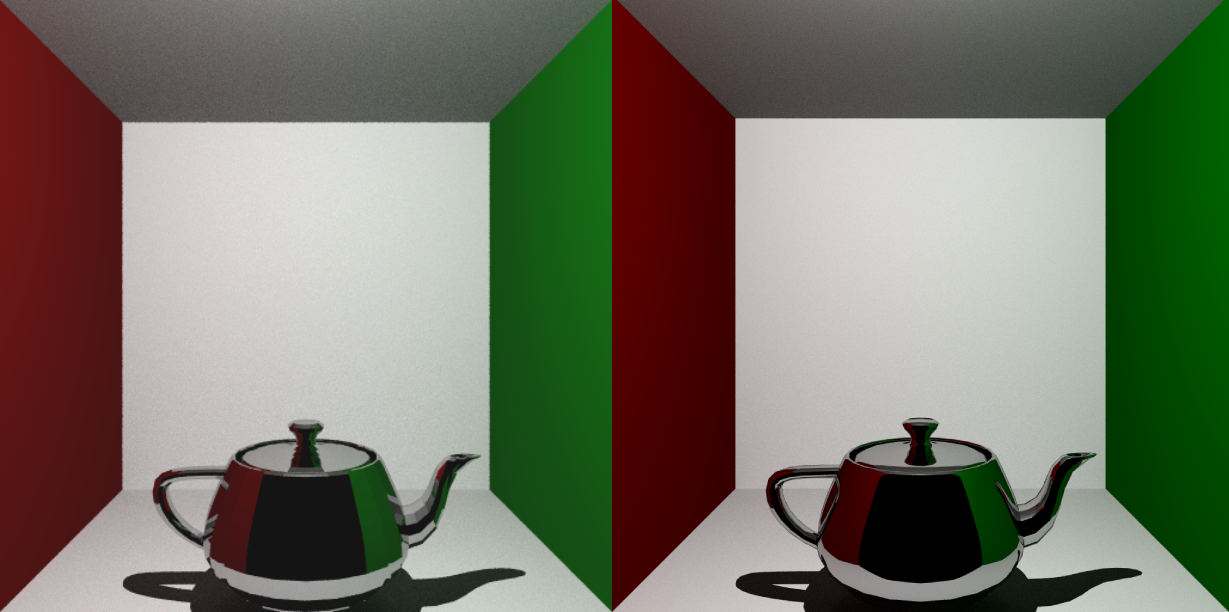
\includegraphics[width = 0.9\textwidth]{images/pmsmoothing.png}
    \caption{Left: An unsmoothed polymesh. Right: A polymesh smoothed using vertex normals.}\label{fig:smoothing}
\end{figure*}

%normal shading
\begin{figure*}[h]
    \centering
    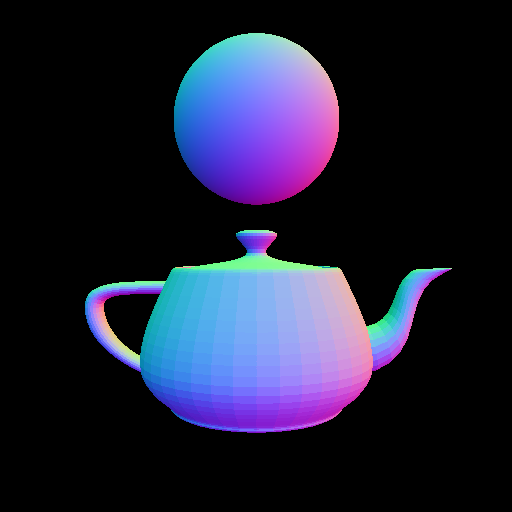
\includegraphics[width = 0.55\textwidth]{images/normalshading.png}
    \caption{Objects with the normal shading material.}\label{fig:normalshading}
\end{figure*}

% image of fresnel on/off for sphere
\begin{figure*}[h]
    \centering
    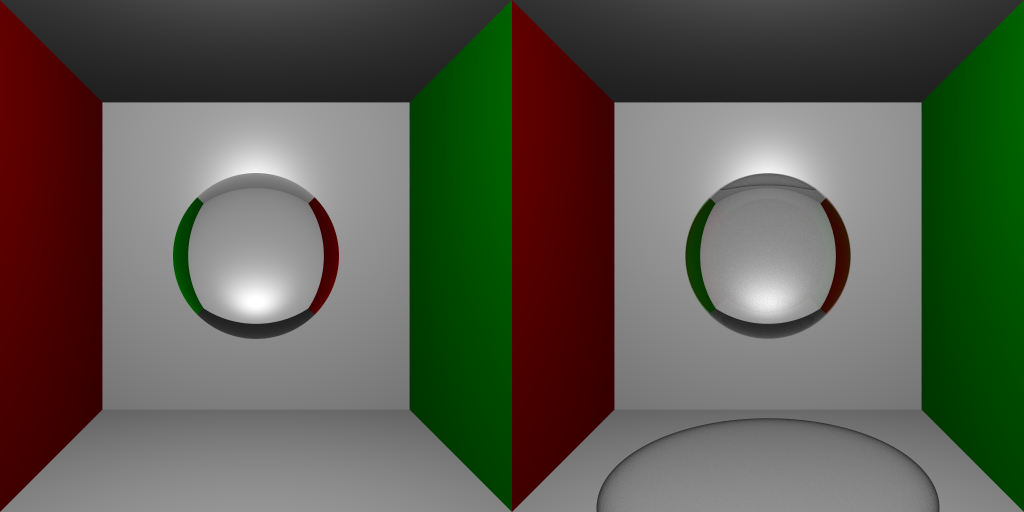
\includegraphics[width = 0.9\textwidth]{images/fresnelcomp.png}
    \caption{Left: No fresnel term, all rays are transmitted. Right: Fresnel term used, some rays near the edges are reflected and a shadow is seen.}\label{fig:fresnel}
\end{figure*}

%  CSGs
\begin{figure*}[h]
    \centering
    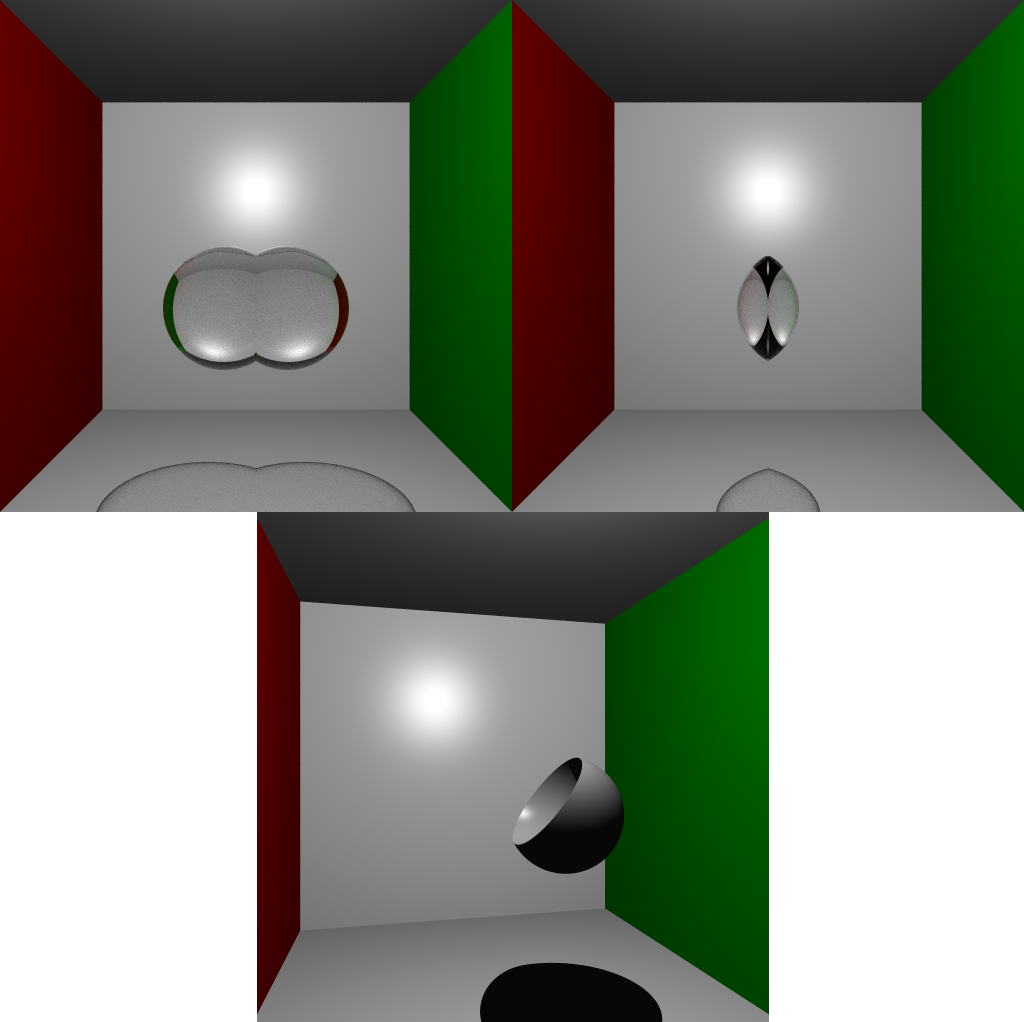
\includegraphics[width = 0.65\textwidth]{images/csgtypes.png}
    \caption{Top Left: Union of glass spheres. Top Right: Intersection of glass spheres. Bottom: Difference of Phong spheres.}\label{fig:csgtypes}
\end{figure*}

%  Quad surface
\begin{figure*}[h]
    \centering
    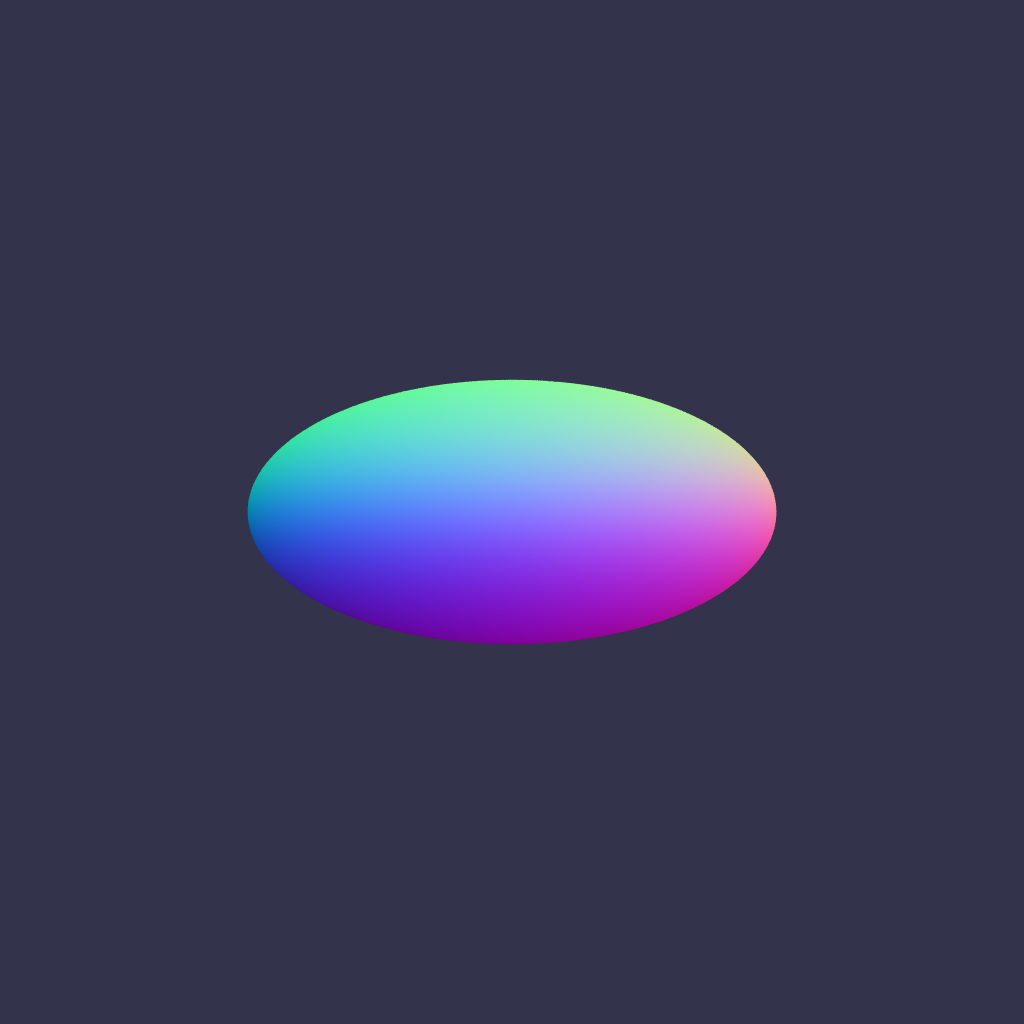
\includegraphics[width = 0.65\textwidth]{images/ellipsoid.png}
    \caption{An ellipsoid with a Phong material.}\label{fig:quadsurface}
\end{figure*}

% depth of field
\begin{figure*}[h]
    \centering
    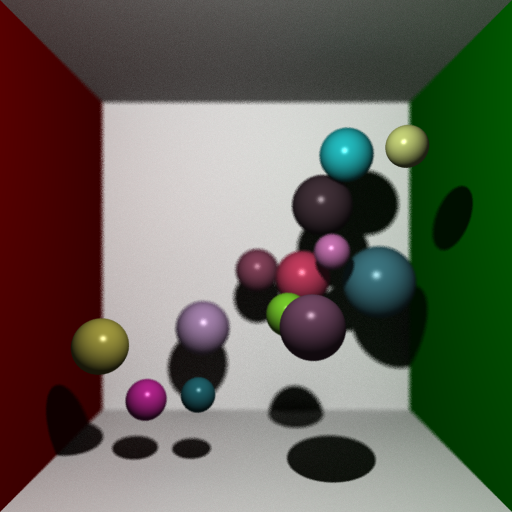
\includegraphics[width = 0.65\textwidth]{images/depthoffield.png}
    \caption{A scene with depth of field: notice how some spheres are blurry and others appear sharp.}\label{fig:depthoffield}
\end{figure*}

% glass shadow good/bad
\begin{figure*}[h]
    \centering
    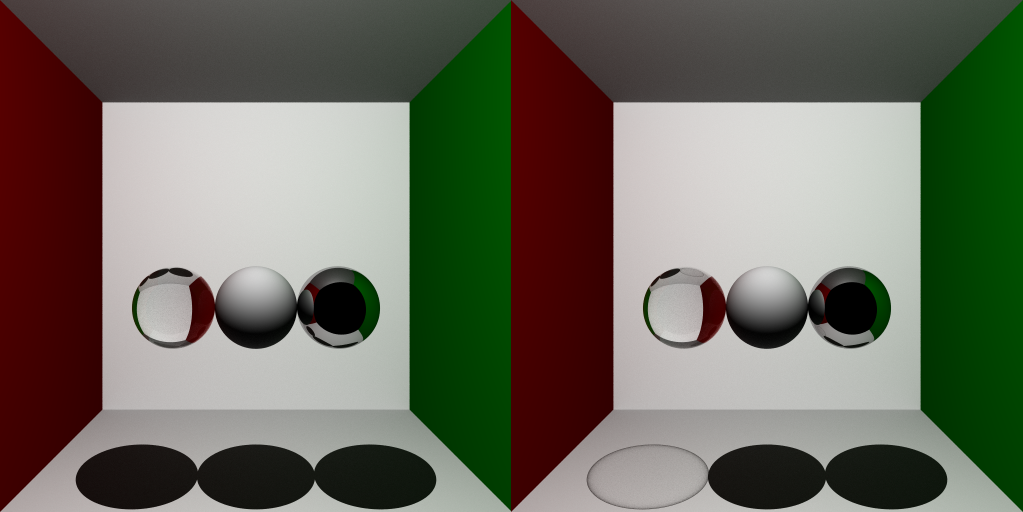
\includegraphics[width = 0.9\textwidth]{images/glassshadow.png}
    \caption{Left: Shadows do not discriminate between materials. Right: Shadows are not created when rays are transmitted by a material.}\label{fig:glassshadow}
\end{figure*}

% photon map
\begin{figure*}[h]
    \centering
    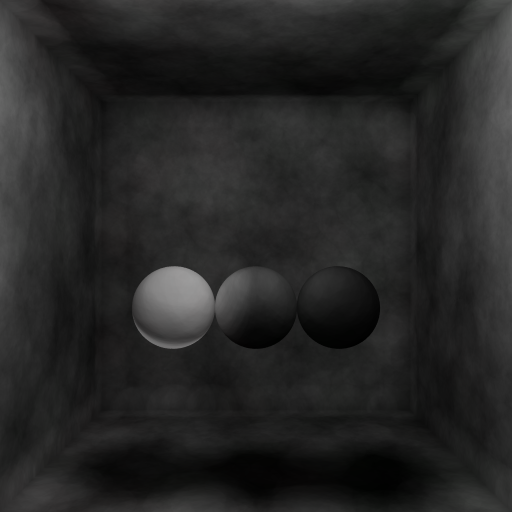
\includegraphics[width = 0.65\textwidth]{images/photonmap.png}
    \caption{Photon map visualisation.}\label{fig:pmap}
\end{figure*}

% photon map
\begin{figure*}[h]
    \centering
    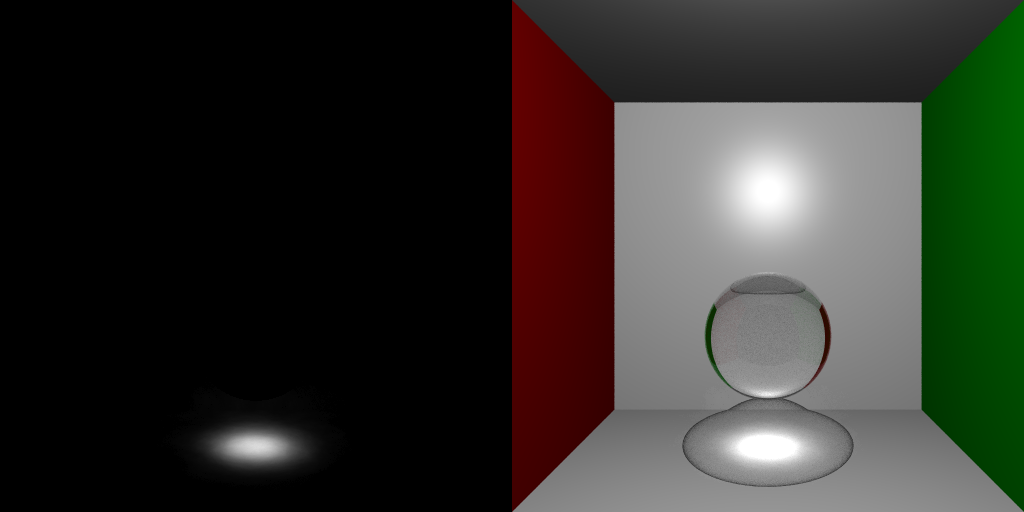
\includegraphics[width = 0.9\textwidth]{images/glassspherecaustics.png}
    \caption{Left: Visualisation of a caustic photon map. Right: Render with caustic visualisation directly added.}\label{fig:glasscaustics}
\end{figure*}

%cognac glass
\begin{figure*}[h]
    \centering
    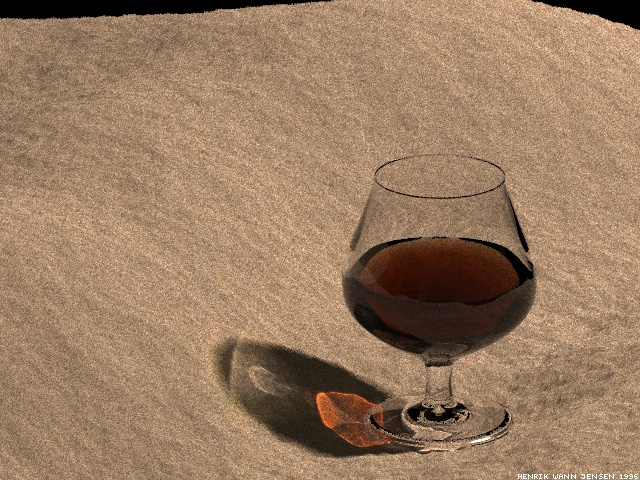
\includegraphics[width = 0.9\textwidth]{images/cognacglass.jpg}
    \caption{A glass of cognac on a fractal surface. The bright parts in the glass' shadow are caustics. Image by Henrik Wann Jensen \cite{Jensen1996photonmaps}.}\label{fig:cognac}
\end{figure*}

\end{document}
